\section{Language Model}\label{sec:model}
Language model

\subsection{Expected Use}
In order to develop the appropriate DSL giving users the power and expressivity they need to easily express usage management concepts, we begin by developing a model describing how we expect it to be used, and by whom, identifying key functional and non-functional characteristics.  We use roles codified as actors to identify the primary user base, and link those roles to specific use cases we expect to be common in day to day DSL use.  We also identify common inputs and outputs from expected activities, and show how those input and output elements are related.  We finally specify the essential core structure of the DSL, as well as extension points and default implementations of those points.

\begin{figure}[!t]
\centering
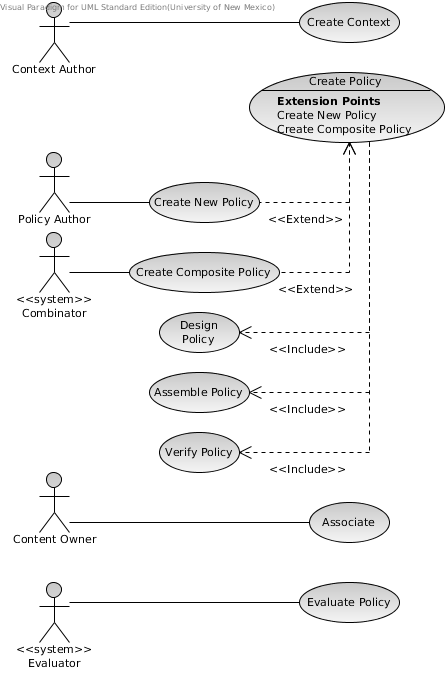
\includegraphics[width=3in]{use-cases}
\caption{General DSL Use Cases}
\label{fig:model:use-cases}
\end{figure}

\subsection{Domain Ontology}

\begin{figure}[!t]
\centering
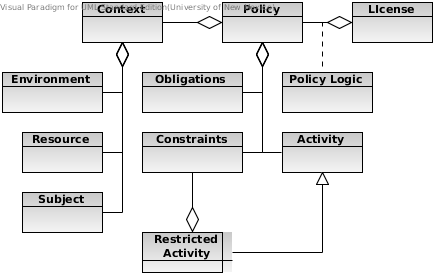
\includegraphics[width=3in]{ontology}
\caption{Basic Language Ontology}
\label{fig:model:ontology}
\end{figure}

\subsection{Envisioned Lifecycle}

\begin{figure}[!t]
\centering
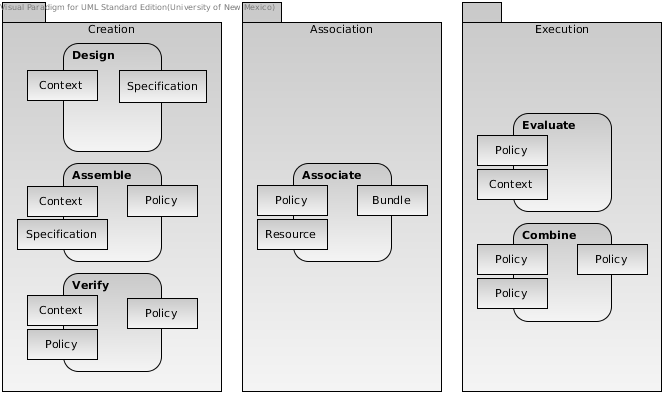
\includegraphics[width=3in]{lifecycle}
\caption{Policy Development Lifecycle}
\label{fig:model:lifecycle}
\end{figure}

\subsection{Language Components}

\begin{figure}[!t]
\centering
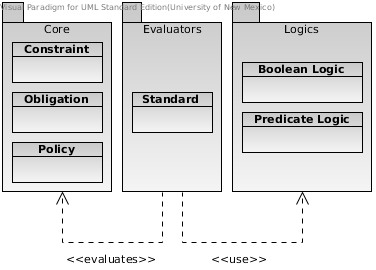
\includegraphics[width=3in]{language-components}
\caption{Language Elements}
\label{fig:model:language-components}
\end{figure}
